% book example for classicthesis.sty
\documentclass[
  % Replace twoside with oneside if you are printing your thesis on a single side
  % of the paper, or for viewing on screen.
  %oneside,
  twoside,
  11pt, a4paper,
  footinclude=true,
  headinclude=true,
  cleardoublepage=empty
]{scrbook}

\usepackage{lipsum}
\usepackage[linedheaders,parts,pdfspacing]{classicthesis}
\usepackage{amsmath}
\usepackage{amsthm}
\usepackage{acronym}
\usepackage{graphicx}

\title{Measurement uncertainties in x-ray computed tomography}
\author{Joshua Greenhalgh}

\begin{document}

\maketitle

%*******************************************************
% Abstract
%*******************************************************
\pdfbookmark[1]{Abstract}{Abstract}
\chapter*{Abstract}

X-ray computed tomography (XCT) is beginning to find a range of new industrial applications. For many years this technique has been applied to non-destructive testing (NDT), however it is now being used by industry for the purpose of metrology. XCT has certain advantages over the traditional approach to metrology that of the coordinate measuring machine (CMM). Foremost among these is the ability to measure both external and internal aspects of an objects geometry without the need to destroy the object. This technique does however suffer from the lack of a clear understanding of the processes metrological uncertainties - if XCT is to be adopted more widely then it is necessary to be able to quantify the underlying uncertainties in this measuring procedure. This Thesis will approach the problem of quantifying these uncertainties via the simulation of an XCT system. The focus will be on the effect of magnification on measurement uncertainty in the presence of realistically modeled source and detector elements.

\textbf{\textit{A previous version of parts of this text was submitted as part of FEEG6018}}

The code used in this project can be found in the code directory of the GitHub repository found at https://github.com/josh-gree/thesis

%*******************************************************
% Table of Contents
%*******************************************************
\pdfbookmark[1]{\contentsname}{tableofcontents}

\setcounter{tocdepth}{2} % <-- 2 includes up to subsections in the ToC
\setcounter{secnumdepth}{3} % <-- 3 numbers up to subsubsections

\tableofcontents

%*******************************************************
% List of Figures and of the Tables
%*******************************************************

%*******************************************************
% List of Figures
%*******************************************************
\pdfbookmark[1]{\listfigurename}{lof}
\listoffigures

%*******************************************************
% List of Tables
%*******************************************************
\pdfbookmark[1]{\listtablename}{lot}
\listoftables
  



\chapter{Introduction}

\begin{table}
\caption{Blah}
\begin{tabular}{c|cccc}
\toprule
{} Magnification &     S0D0 &     S1D0 &     S0D1 &     S1D1 \\
\midrule
1.5000        &  29.9141 &  29.8956 &  29.8804 &  29.8763 \\
1.7778        &  29.8963 &  29.8871 &  29.8834 &  29.8776 \\
2.0556        &  29.9046 &  29.8858 &  29.8867 &  29.8785 \\
2.3333        &  29.9105 &  29.8859 &  29.8913 &  29.8796 \\
2.6111        &  29.9020 &  29.8845 &  29.8929 &  29.8795 \\
2.8889        &  29.8946 &  29.8828 &  29.8927 &  29.8788 \\
3.1667        &  29.9036 &  29.8814 &  29.8940 &  29.8782 \\
3.4444        &  29.9057 &  29.8805 &  29.8957 &  29.8776 \\
3.7222        &  29.9034 &  29.8794 &  29.8957 &  29.8771 \\
4.0000        &  29.9000 &  29.8781 &  29.8955 &  29.8760 \\
\bottomrule
\end{tabular}
\end{table}

\chapter{Litrature Review}
\section{Metrology}
\section{Computed Tomography}
\section{Simulation}
\chapter{Experimental Methodolgy}
\section{Spherical Projections}
\section{Beam Hardening}
\chapter{Results}

\begin{figure}[h!]
  \caption{Blah}
  \centering
    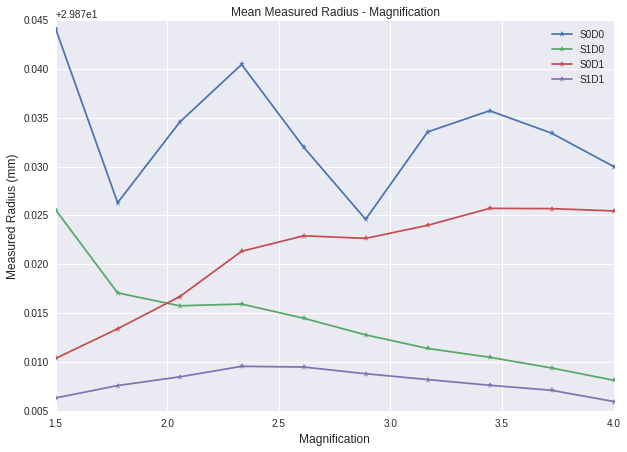
\includegraphics[width=\textwidth]{figures/output_6_0.png}
\end{figure}


\section{Measurement Uncertainty}
\section{Image Resolution}
\section{Analytic MTF}
\chapter{Conclusion}




\end{document}
